\documentclass{standalone}
\usepackage{tikz}
\usetikzlibrary{calc,shapes.multipart,chains,arrows}

\begin{document}

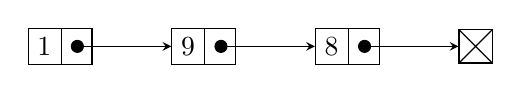
\begin{tikzpicture}[list/.style={rectangle split, rectangle split parts=2,
    draw, rectangle split horizontal}, >=stealth, start chain]

  \node[list,on chain] (A) {1};
  \node[list,on chain] (B) {9};
  \node[list,on chain] (C) {8};
  \node[on chain,draw,inner sep=6pt] (D) {};
  \draw (D.north east) -- (D.south west);
  \draw (D.north west) -- (D.south east);
  \draw[*->] let \p1 = (A.two), \p2 = (A.center) in (\x1,\y2) -- (B);
  \draw[*->] let \p1 = (B.two), \p2 = (B.center) in (\x1,\y2) -- (C);
  \draw[*->] let \p1 = (C.two), \p2 = (C.center) in (\x1,\y2) -- (D);
\end{tikzpicture}

\end{document}